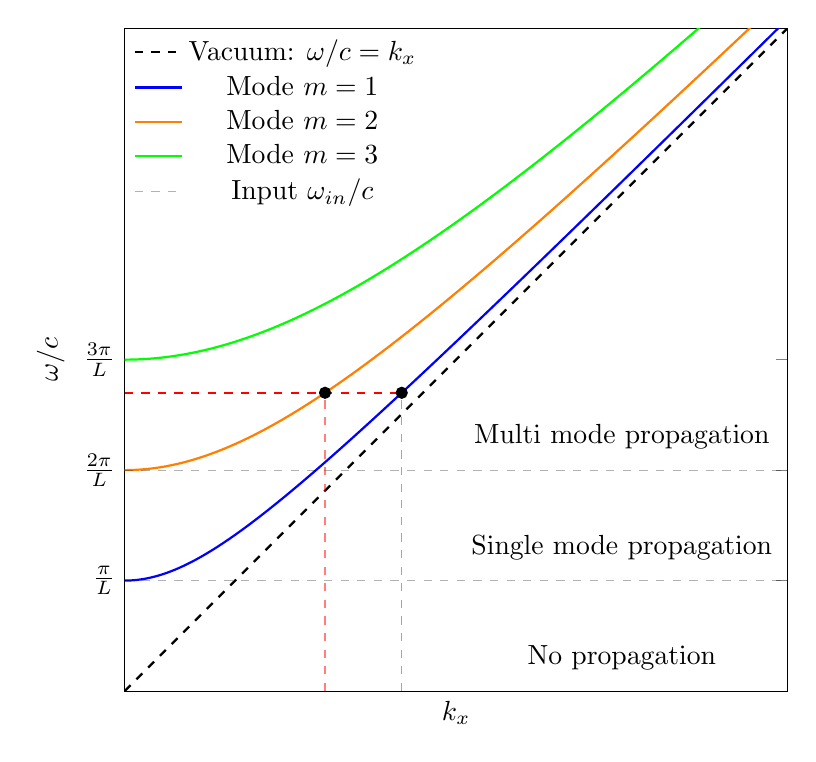
\begin{tikzpicture}
\begin{axis}[
    width=10cm,
    height=10cm,
    xlabel={$k_x$},
    ylabel={$\omega / c$},
    xmin=0, xmax=6,
    ymin=0, ymax=6,
    xtick=\empty,
    ytick={1,2,3},
    yticklabels={
        $\frac{\pi}{L}$,
        $\frac{2\pi}{L}$,
        $\frac{3\pi}{L}$
    },
    legend style={
    at={(0,1)},      % x=0 (left), y=1 (top)
    anchor=north west,
    draw=none,
    fill=none
    },
    domain=0:6,
    samples=200
]

% -----------------------------
% Vacuum dispersion
% -----------------------------
\addplot[
    dashed,
    thick
] {x};
\addlegendentry{Vacuum: $\omega/c = k_x$}

% -----------------------------
% Mode dispersions
% -----------------------------
\addplot[thick, blue]{sqrt(x^2 + 1^2)};
\addlegendentry{Mode $m=1$}
\addplot[thick, orange]{sqrt(x^2 + 2^2)};
\addlegendentry{Mode $m=2$}
\addplot[thick, green]{sqrt(x^2 + 3^2)};
\addlegendentry{Mode $m=3$}

% -----------------------------
% Horizontal cutoff lines
% -----------------------------
\foreach \m in {1,2} {
    \addplot[
        dashed,
        black,
        opacity=0.3
    ] coordinates {(0,\m) (6,\m)};
}

% -----------------------------
% Input frequency line
% -----------------------------
\def\omegain{2.7}

\addplot[
    dashed,
    thick,
    red
] coordinates {(0,\omegain) (2.5,\omegain)};
\addlegendentry{Input $\omega_{\text{in}}/c$}

% -----------------------------
% Excited mode intersections
% Solve sqrt(k^2 + m^2) = omegain
% => k = sqrt(omegain^2 - m^2)
% -----------------------------
\foreach \m in {1,2} {
    \pgfmathsetmacro{\kx}{sqrt(\omegain^2 - \m^2)}

    \addplot[
        only marks,
        mark=*,
    ] coordinates {(\kx,\omegain)};

    \addplot[
        dashed,
        opacity=0.5,
        red
    ] coordinates {(\kx,0) (\kx,\omegain)};
}

% -----------------------------
% Region labels
% -----------------------------
\node at (axis cs:4.5,0.3) {No propagation};
\node at (axis cs:4.5,1.3) {Single mode propagation};
\node at (axis cs:4.5,2.3) {Multi mode propagation};

\end{axis}
\end{tikzpicture}

